
% ===========================
\chapter{Konzept}
\label{konzept}
% ===========================

Wie in Abschnitt \ref{grundlagen_fahren} beschrieben, stellt die Absicherung von hochautomatisierten \ac{FAS} die Automobilindustrie vor große Herausforderungen. Die Menge der bekannten Fahrszenarien ist nur eine Teilmenge aller Szenarien, die zukünftige \ac{FAS} abdecken müssen. Die Folge ist eine steigende Anzahl benötigter Testkilometer, die in Zukunft mit ökonomischem Aufwand nicht mehr umsetzbar sein wird. Es müssen neue Methoden gefunden werden, relevante Szenarien für die Generierung von Testfällen zu identifizieren, um die Sicherung von hochautomatisierten \ac{FAS} mit ökonomischen Aufwand garantieren zu können.

Genau hier soll diese Arbeit einen Beitrag liefern. Das Ziel, wie bereits in Abschnitt \ref{einleitung_zielsetzung} erklärt, ist die Klassifizierung von realen Fahrszenarien. Die Grundidee ist es, einen Klassifikator mit einem großen Anteil synthetischer Daten und einem kleinen Anteil realer Daten von bisher bekannten Szenarien zu trainieren. Es wird mit einem großen Teil synthetischer Daten gearbeitet, weil es in der Praxis einfacher ist, synthetische Daten zu generieren und automatisch zu annotieren als große Mengen realer Daten zu annotieren. Die Idee ist, dass auf diese Weise auch unbekannte Szenarien herausgefiltert werden können, weil diese von dem trainierten Klassifikator nicht erkannt werden. Diese bisher unbekannten Szenarien können dann wiederum als Basis für neue Testfälle für die Sicherung hochautomatisierter Fahrfunktionen verwendet werden.

In dieser Arbeit soll ein Proof-of-Concept für diese Methodik entwickelt werden. Dafür wird im folgenden Abschnitt \ref{konzept_struktur} das Konzept im Detail und die Vorgehensweise vorgestellt. Anschließend werden in Abschnitt \ref{konzept_methodik} die Ansätze, Methoden und Werkzeuge für die Umsetzung aufgelistet.


% ===========================
\section{Struktur}
\label{konzept_struktur}
% ===========================

Das Konzept dieser Arbeit lässt sich in vier Teile untergliedern. Im ersten Teil werden beispielhaft einige Szenarien ausgewählt und auf der Ebene der \textit{logischen Szenarien} definiert. Auf dieser Basis werden im zweiten Teil synthetische und reale Trainingsdaten generiert. Im dritten Teil wird ein \ac{KNN} als Klassifikator trainiert und evaluiert. In einem vierten Schritt können die Schritte 1 bis 3 mit allen bekannten Szenarien wiederholt werden um bisher unebkannte Szenarien zu finden. Die ersten drei Schritte, die in dieser Arbeit als Proof-of-Concept umgesetzt werden, ist schematisch in Abbildung \ref{fig_konzept_struktur} dargestellt. In den folgenden Absätzen werden die Schritte im Detail beschrieben.

\begin{figure}[h]
\centering
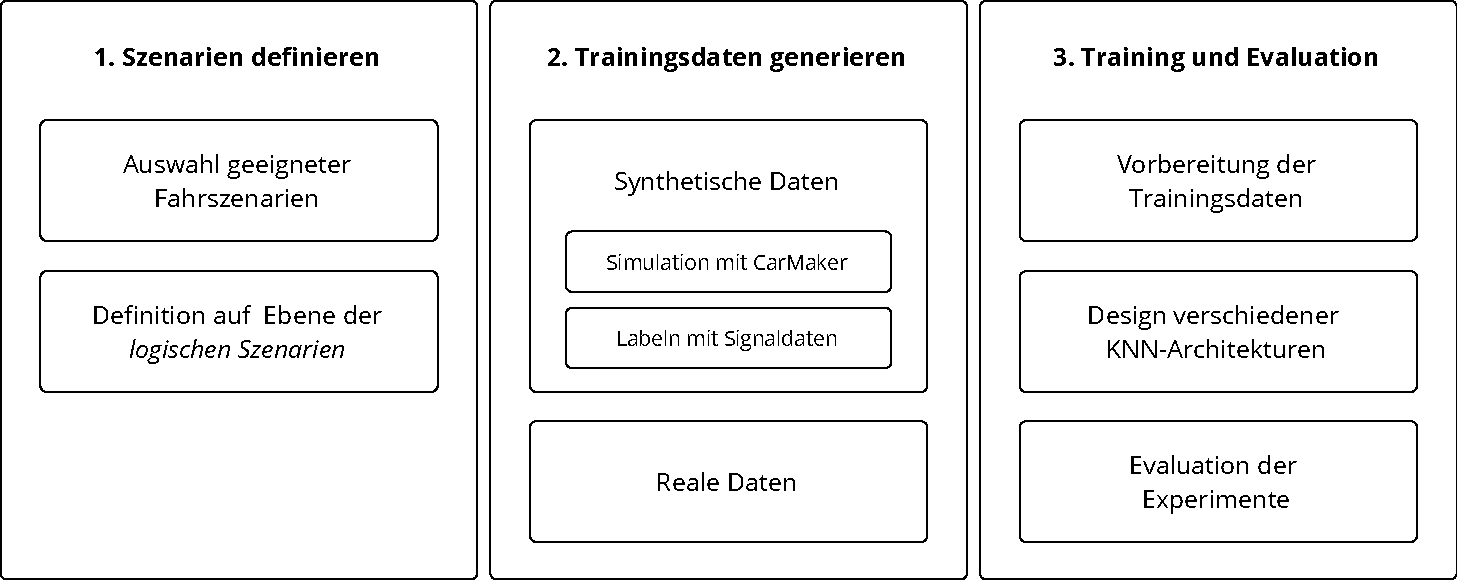
\includegraphics[scale=0.6]{images/konzept_struktur.pdf}
\caption{Konzept dieser Arbeit}
\label{fig_konzept_struktur}
\end{figure}

Im ersten Schritt werden beispielhaft Fahrszenarien ausgewählt und wie in Abschnitt \ref{grundlagen_fahren_szenarien} definiert. In dieser Arbeit werden Szenarien auf der Ebene der \textit{logischen Szenarien} definiert. Nachdem Szenarien ausgewählt und definiert sind, werden synthetische und reale Daten für das Training eines Klassifikators benötigt.

Für die Generierung von synthetischen Daten wird mit einer Simulationssoftware gearbeitet. Die Idee ist es, Fahrten eines Ego-Fahrzeugs zu simulieren, entsprechende Bild- und Signaldaten aufzuzeichnen und die Bilddaten anhand der Signaldaten zu annotieren. Auf diese Weise können ohne großen Aufwand beliebig viele synthetische Daten erzeugt und annotiert werden. Amersbach und Winner \cite{amersbach2017functional} stellen einen Ansatz für die funktionale Dekomposition von hochautomatisierten \ac{FAS} vor. In diesem Ansatz werden Informationen über sechs Schichten, von den Ground Truth Daten über die Szenenerkennung bis zur entsprechenden Aktion des Ego-Fahrzeugs, abgeleitet. Ein Schema dieses Ansatzes ist in Abbildung \ref{fig_functional_decomposition} dargestellt. In dieser Arbeit werden für die Annotation der Bilddaten Signaldaten generiert, die nach Schicht 1 (e.g. Geschwindigkeit des Ego-Fahrzeugs) und Schicht 2 (e.g Position des vorausfahrenden Fahrzeugs) eingeordnet werden können. Jeder generierte Zeitpunkt stellt eine Szene, wie in Abschnitt \ref{grundlagen_fahren_szenarien} beschrieben, dar. Jede Szene wird separat auf Basis der entsprechenden Signaldaten nach festgelegten Regeln annotiert. Die Aneinanderreihung von mehreren Szenen ergibt schließlich ein Szenario. Für die Generierung von realen Trainingsdaten werden aufgezeichnete Videos manuell annotiert.

\begin{figure}[h]
\centering
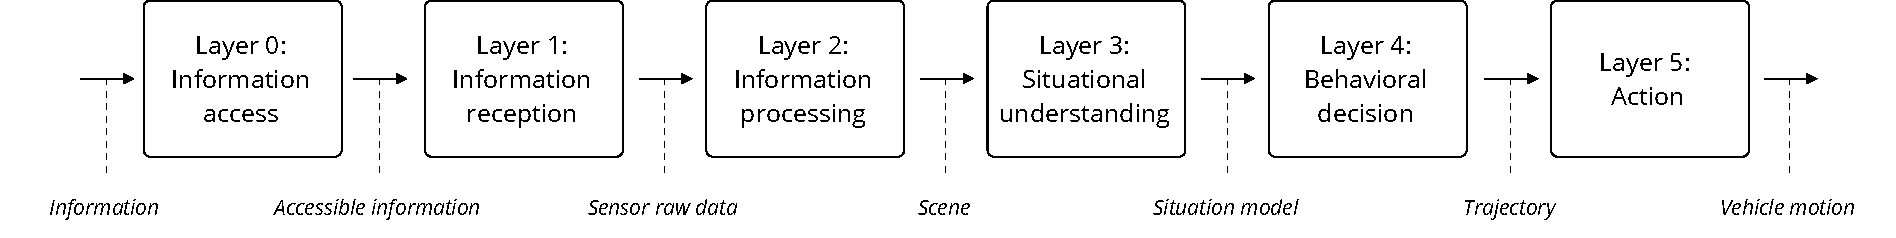
\includegraphics[scale=0.45]{images/funktionale_dekomposition.pdf}
\caption[Schema der funktionalen Dekomposition]{Schema der funktionalen Dekomposition \cite{amersbach2017functional}}
\label{fig_functional_decomposition}
\end{figure}

In dieser Arbeit sollen \acp{KNN} als Klassifikators verwendet werden. Wie in Abschnitt \ref{grundlagen_nn_video} beschrieben, gibt es verschiedene Ansätze wie ein Klassifikator für Videos trainiert werden kann. In dieser Arbeit werden zwei verschiedene Ansätze angewendet und miteinander verglichen. Beim ersten Ansatz werden \acp{CNN} verwendet, um einzelne Bilder zu klassifizieren. Mit dem zweiten Ansatz wird ein Klassifikator aus einer Kombination von \acp{CNN} und \acp{LSTM} erstellt. Wie oben beschrieben wird für das Training nur ein kleiner Teil realer und ein großer Teil synthetischer Daten verwendet, um die Skalierbarkeit dieses Ansatzes in der Praxis zu gewährleisten.

Der Proof-of-Concept in dieser Arbeit ist erfolgreich, wenn ein Klassifikator mit diesen drei Schritte trainiert werden und im Anschluss Szenarien auf Basis von Bilddaten klassifizieren kann. Danach kann in einem vierten Schritt ein weiterer Klassifikator mit allen bisher bekannten Szenarien nach demselben Prinzip trainiert werden. Dieser Klassifikator kann im Anschluss alle bisher bekannten Szenarien klassifizieren und bisher unbekannte Szenarien herausfiltern, wenn beispielsweise eine Schwelle für die Klassifizierungsgenauigkeit unterschritten wird. Damit wird es möglich die Menge der bisher bekannten Szenarien zu erweitern und die Absicherung von hochautomatisierten \ac{FAS} weiter voranzutreiben.

% ===========================
\section{Ansätze, Methoden, Werkzeuge}
\label{konzept_methodik}
% ===========================

In diesem Abschnitt wird ein Überblick gegeben, welche Ansätze, Methoden und Werkzeuge in den jeweiligen Teilen der Umsetzung verwendet werden. Diese Zuordnung ist in der folgenden Tabelle \ref{tab_konzept_methods} dargestellt. Die detaillierte Beschreibung folgt in Kapitel \ref{umsetzung}.

\begin{longtable}[c]{p{5cm} p{6.5cm} p{1.5cm}}
\textbf{Teil der Umsetzung} & \textbf{Ansätze, Methoden, Werkzeuge} & \textbf{Quellen} \\
\hline
\endhead

Auswahl und Definition geeigneter Fahrszenarien & Konzept der \textit{logischen Szenarien} & \cite{ulbrich2015defining}, \cite{bagschik2017szenarien} \\
\hline
Simulation und Annotation synthetischer Trainingsdaten & Generierung von Bild- und Signaldaten mit CarMaker, regelbasierte Klassifizierung auf Basis von vorher festgelegten Signaldaten & \cite{ipg2018carmaker} \\
\hline
Generierung realer Trainingsdaten & Auswahl geeigneter Videosequenzen von YouTube, manuelle Annotation & \cite{youtube2018video}, \cite{google2018route1}, \cite{google2018route2} \\
\hline
Vorbereitung der Daten, Erstellung des Klassifikators und Evaluation der Experimente & Verschiedene Architekturen mit \acp{CNN} und \acp{LSTM}, implementiert mit Python und Keras & \cite{chollet2015keras}, \cite{lecun2010convolutional}, \cite{hochreiter1997long} \\

\hline
\caption{Ansätze, Methoden und Werkzeuge dieser Arbeit}
\label{tab_konzept_methods}
\end{longtable}




